\documentclass[11pt,aspectratio=169]{beamer}
\usepackage[T1]{fontenc}
\usepackage{lmodern}
\usepackage{amsmath,amssymb,booktabs,graphicx}
\definecolor{Ink}{HTML}{23313D}
\definecolor{Accent}{HTML}{126B75}
\definecolor{Muted}{HTML}{67737C}
\definecolor{Warm}{HTML}{AD591D}
\setbeamercolor{normal text}{fg=Ink,bg=white}
\setbeamercolor{structure}{fg=Accent}
\setbeamercolor{frametitle}{fg=Ink}
\setbeamercolor{alerted text}{fg=Warm}
\setbeamerfont{frametitle}{size=\Large,series=\bfseries}
\setbeamerfont{title}{size=\LARGE,series=\bfseries}
\setbeamersize{text margin left=8mm,text margin right=8mm}
\setbeamertemplate{navigation symbols}{}
\setbeamertemplate{itemize item}{\small\raise1pt\hbox{\textcolor{Accent}{\textbullet}}}
\setbeamertemplate{frametitle}{\vspace{3mm}\insertframetitle\par\vspace{1mm}{\color{Accent}\hrule height .5pt}\vspace{2mm}}
\setbeamertemplate{footline}{\hspace{8mm}\textcolor{Muted}{\scriptsize Acemoglu, Kong \& Ozdaglar (2026)}\hfill\textcolor{Muted}{\scriptsize\insertframenumber\,/\,\inserttotalframenumber}\hspace{8mm}\vspace{3mm}}
\newcommand{\source}[1]{\par\vspace{2mm}{\scriptsize\color{Muted}#1}}
\newcommand{\claim}[1]{{\color{Accent}\bfseries #1}\par\medskip}
\newcommand{\photopanel}[1]{%
\IfFileExists{#1}{\includegraphics[width=\linewidth,height=4.05cm,keepaspectratio]{#1}}{%
\fbox{\begin{minipage}[c][3.8cm][c]{.88\linewidth}\centering
\textcolor{Warm}{\textbf{Handwritten photo pending}}\par\medskip
\small Derive $g'$, $U_{eX}$ and $U_{e\tau_A}$ on paper.\par\medskip
Photograph your work and save it as\par\texttt{hand/derivation.jpg}.\par\medskip
\scriptsize This panel is not evidence of handwritten work.
\end{minipage}}}}

\title{Better advice, weaker learning?}
\subtitle{AI, Human Cognition and Knowledge Collapse}
\author{Daron Acemoglu, Dingwen Kong and Asuman Ozdaglar}
\date{NBER Working Paper 34910 \enspace / \enspace February 2026}
\begin{document}
\begin{frame}
\vspace{5mm}
{\color{Accent}\small STATIC INCENTIVES $\longrightarrow$ COLLECTIVE KNOWLEDGE}\par\bigskip
{\usebeamerfont{title}\inserttitle}\par\medskip
{\large\insertsubtitle}\par\bigskip
\insertauthor\par\smallskip
{\small\color{Muted}\insertdate}\par\bigskip
\href{https://github.com/gsaco/ai-04-acemoglu}{\textcolor{Accent}{github.com/gsaco/ai-04-acemoglu}}
\source{Five-minute discussion. Focus: static problem and Observation 1.}
\end{frame}

\begin{frame}{1 \enspace The paper and the agent's problem}
\claim{Can better individual advice weaken the knowledge everyone needs?}
\[
\max_{e\geq0}\ U(e;X,\tau_A)
=G(X)\Delta_G+G(X)G(Y)\Delta_X-\frac{e^\alpha}{\alpha},
\qquad Y=\sigma^{-2}+\lambda_I e+\tau_A.
\]
\begin{itemize}\setlength\itemsep{2mm}
\item $X$: inherited public precision; $Y$: context-specific precision.
\item $G(z)=2\Phi(\sqrt z)-1$: probability the prediction error is within 1.
\item Effort produces private information and a public spillover; short-lived,
atomistic agents take $X$ as given.
\end{itemize}
\medskip
\textbf{Production restriction:} $\Delta_I=0$, $\Delta_X>0$, $\Delta_G+\Delta_X=1$.
\source{Source: \S\S3.1--3.3, pp. 7--12, eqs. (4)--(6); constant $f(0,0)$ omitted.\newline
The supplied paper's \S2 is related literature; its static model starts in \S3.}
\end{frame}

\begin{frame}{2 \enspace Observation 1: two signs, explicit conditions}
\[
g(z)=\frac{\phi(\sqrt z)}{\sqrt z},\qquad
 g'(z)=-\frac12(1+z^{-1})g(z)<0.
\]
\[
\underbrace{U_{eX}=\Delta_X\lambda_I g(X)g(Y)>0}_{\text{general knowledge complements effort}}
\qquad
\underbrace{U_{e\tau_A}=\Delta_XG(X)\lambda_I g'(Y)<0}_{\text{agentic advice substitutes for effort}}
\]
\small
\textbf{Conditions:} $X>0$, finite $\tau_A\geq0$, $\sigma^{-2}>0$, $\lambda_I>0$,
$\alpha>1$; Assumption 1, independent Gaussian information, unit-tolerance payoffs;
public learning is not privately internalized.
\medskip

$U_{ee}<0$ gives a unique interior optimum: $e_X^*>0$, $e_{\tau_A}^*<0$.
At $X=0$, $e^*=0$; the strict interior statements do not apply.
\medskip

\textbf{Welfare caution:} fixed-$X$ utility rises; long-run welfare need not.
The single-peak claims require $\sigma^{-2}\geq\sqrt2-1$ and the relevant
$\alpha-1\gtrless1/4$ regime; the optimum may be $\tau_A^*=0$.
\source{Source: Observation 1, p. 13; Observation 2, p. 14; Propositions 10--11, p. 26.}
\end{frame}

\begin{frame}{3 \enspace What I did: verify signs, test the hidden premise}
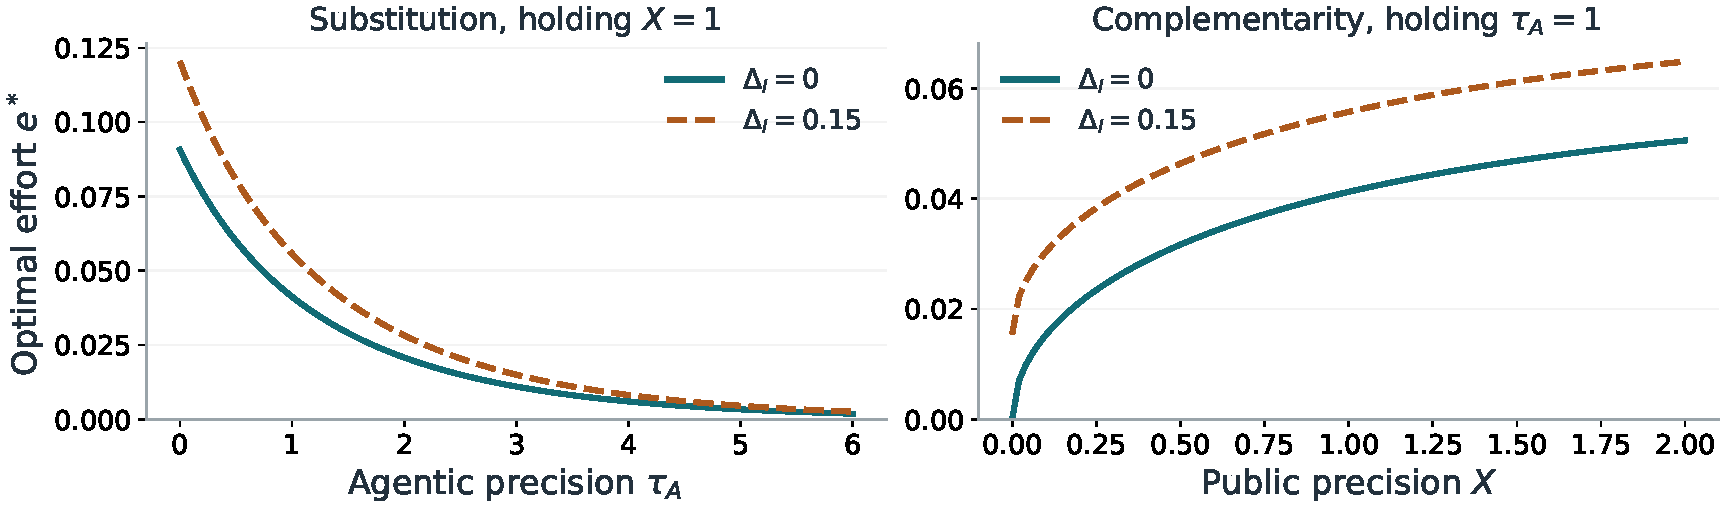
\includegraphics[width=\textwidth,height=3.5cm,keepaspectratio]{extra/figures/static_checks.pdf}\par
\small
\textbf{Reproducible static checks:} SymPy identities + 444 numerical optima;
maximum FOC residual $<2.5\times10^{-15}$.
\medskip

\textbf{Extension:} allow $\Delta_I=0.15$. Both signs survive, but at $X=0$,
$\tau_A=1$, effort rises from $0$ to $0.01539$.
\source{Own AI-assisted analysis in extra/static\_checks.py; $\alpha=2$, $\lambda_I=1$, $\sigma^{-2}=1$, $\Delta_X=.6$;
$\Delta_G=1-\Delta_I-\Delta_X$. No dynamic results simulated.}
\end{frame}

\begin{frame}{4 \enspace Where I challenged the AI's reasoning}
\begin{columns}[T]
\begin{column}{.43\textwidth}
\photopanel{hand/derivation.jpg}
\end{column}
\begin{column}{.53\textwidth}
\small
\textbf{Claim tested:} ``More accurate AI must raise welfare.''
\medskip

\textbf{Verdict:} true for optimized static utility at fixed $X$; not a general
long-run conclusion. Public-knowledge losses also matter.
\medskip

\textbf{The assumption audit:} \S5 relaxes aggregation, synthetic data and effort bundling.
It retains $\Delta_I=0$.
\[
 U_e\big|_{X=0,e=0}=\Delta_I\lambda_I
 g(\sigma^{-2}+\tau_A)>0
\]
\textbf{My extension:} with $\Delta_I>0$, private learning remains valuable at $X=0$.
\end{column}
\end{columns}
\source{Source: Assumption 1, p. 8; \S4.3, pp. 24--26; \S5, pp. 29--32.}
\end{frame}
\end{document}
